\section[Probability Refresher II]{Probability Refresher II \small{\textit{2014-04-25}}}

\subsection{Rules of Probability}
Assume a hat filled with cards. Each card has a red and a blue side, the red sides 
are labeled from 1 to 6 and blue sides from 1 to 4, resulting in 24 different cards.
We can describe this \textbf{sample space} (or \textit{set of all possible outcomes}) 
\textbf{$\Omega$} with
\begin{align*}
\Omega = \left\{ \left[ 1, 1\right], \left[ 1, 2\right], ..., \left[ 6, 4\right] \right\}
\end{align*}
where $\left[ 1, 2 \right]$ represents the card with 1 on the red and 2 on the blue side.

To describe the following examples we first have to define some terms and relations.

\begin{itemize}
	\item $x \in \Omega$ is the \textbf{random variable} $x$ which can be drawn from $\Omega$.
    \begin{itemize}
      \item Example: $\left[ 1, 2 \right]$, i.e. the card with a red 1 and a blue 2.
    \end{itemize}
  \item $|S|$ where $S$ is a set is the \textbf{number of elements} in $S$.
    \begin{itemize}
      \item Example: $|\left\{1,2\right\}| = 2$
    \end{itemize}
  \item $E \subset \Omega$ is an \textbf{Event} $E$ (\textit{something you can bet on}).
    \begin{itemize}
      \item Example: Drawing a card with the number on the red site smaller than number on the blue site.
    \end{itemize}
\end{itemize}

How many events do we have? The number of events is simply $2^{|\Omega|} = 2^{24} 
= 2^{10} * 2^{10} * 2^4 \approx 16\mbox{ Mio}$.

If we now put another $\left[ 1, 1\right]$ card into the hat, the \textit{number of events stays the same, but the probabilities change}. This can be seen in the following table \ref{tab:2014-04-25_cards}.

\begin{table}[ht]
	\centering
    \begin{tabular}{cc|*{6}{c|}}
      \cline{3-8}
                                                  &   & \multicolumn{6}{ c| }{red}                                                                          \\ \cline{3-8}
                                                  &   & 1              & 2              & 3              & 4              & 5              & 6              \\ \cline{1-8}
      \multicolumn{1}{|c|}{\multirow{4}{*}{blue}} & 1 & $\frac{2}{25}$ & $\frac{1}{25}$ & $\frac{1}{25}$ & $\frac{1}{25}$ & $\frac{1}{25}$ & $\frac{1}{25}$ \\ \cline{2-8}
      \multicolumn{1}{|c|}{}                      & 2 & $\frac{1}{25}$ & $\frac{1}{25}$ & $\frac{1}{25}$ & $\frac{1}{25}$ & $\frac{1}{25}$ & $\frac{1}{25}$ \\ \cline{2-8}
      \multicolumn{1}{|c|}{}                      & 3 & $\frac{1}{25}$ & $\frac{1}{25}$ & $\frac{1}{25}$ & $\frac{1}{25}$ & $\frac{1}{25}$ & $\frac{1}{25}$ \\ \cline{2-8}
      \multicolumn{1}{|c|}{}                      & 4 & $\frac{1}{25}$ & $\frac{1}{25}$ & $\frac{1}{25}$ & $\frac{1}{25}$ & $\frac{1}{25}$ & $\frac{1}{25}$ \\ \cline{1-8}
\end{tabular}
	\caption{Probabilities of drawing a specific card from the hat}
	\label{tab:2014-04-25_cards}
\end{table}

To get the probability of an event we just have to sum up the values in table 
\ref{tab:2014-04-25_cards}. For example for the event ``The red number is smaller 
than the blue number'', let's call it $R < B$, the probability $P(R < B)$ can be 
calculated as follows:

\begin{align*}
P(R < B) &= P(R=1, B=2) + P(R=1, B=3) + P(R=2, B=3) \\
         &+ P(R=1, B=4) + P(R=2, B=4) + P(R=3, B=4) \nonumber \\
         &= 6 \cdot \frac{1}{25} = \frac{6}{25}
\end{align*}



\subsection{Axioms of Probability}
\begin{description}
	\item[1.] $P({}) = 0, P(\Omega) = 1$
  \item[2.] $\forall E: 0 \leq P(E) \leq 1$
  \item[3.] if $E = E_1 \cup E_2 \wedge E_1 \cap E_2 = \left\{ \right\}$ 
            then $P(E) = P(E_1 \cup E_2) = P(E_1) + P(E_2)$
  \item[3'.] \textit{(follows from 3)} 
            if $E = \bigcup_{i=1}^n E_i \  \wedge \ \forall_{i, j; i \neq j} E_i \cap E_j = \left\{ \right\}$
            then $P(E) = P(\bigcup_{i=1}^n E_i) = \sum_{i=1}^{n}{P(E_i)}$
\end{description}

We can calculate $P$ for all events by adding up singleton events.

\subsubsection*{Other rules that follow}
\begin{figure}[ht]
  \begin{center}
    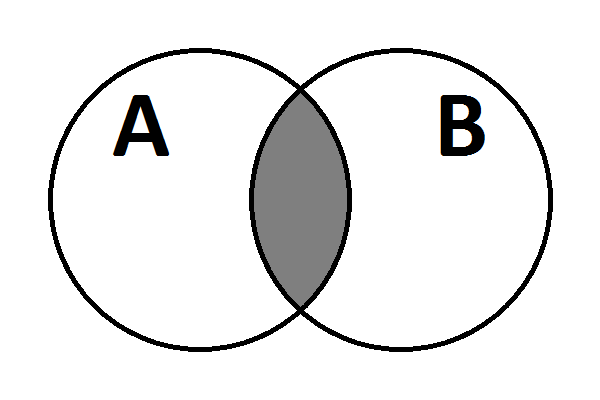
\includegraphics[scale=0.3]{venn_diagram_a_intersects_b}
    \caption{The intersection between two sets makes math a bit tricky}
    \label{fig:venn_a_inter_b}
  \end{center}
\end{figure}

\begin{align*}
& P(A \cup B) = P(A) + P(B) - P(A \cap B) = P(A \setminus B) + P(A \cap B) + P(B \setminus A)\\
& P(A \cup \neg A) = P(\Omega) = 1 = P(A) + P(\neg A)\\
& P(A) = 1- P(\neg A)
\end{align*}



\subsection{Random Variables \& Joint Distribution}
An example for a joint distribution: You roll two dice, one is six-sided and red, the other one is four sided and blue.
\begin{align*}
\mbox{R: }\Omega_R = \{1, ..., 6\} & & P(R=\omega) = \frac{1}{6}\ \forall\ \omega \in \Omega_R\\
\mbox{B: }\Omega_B = \{1, ..., 4\} & & P(B=\omega) = \frac{1}{4}\ \forall\ \omega \in \Omega_B
\end{align*}
The joint sample space $\Omega$ is $\Omega = \Omega_R \times \Omega_B$.

Since R and B are independent the joint probability is $ P(R, B) = \frac{1}{24}$ for all value of R, B.

More formally speaking it holds that $P(R=i, B=j) = \frac{1}{24}$ for all values of $i, j$ since $P(R, B) = P(R) \cdot P(B)$ for all independent $R, B$.
\subsection{Marginal and Conditional Probability}


\subsubsection*{Marginal Probability}


\subsubsection*{Conditional Probability}